\documentclass[]{article}
\usepackage{lmodern}
\usepackage{amssymb,amsmath}
\usepackage{ifxetex,ifluatex}
\usepackage{fixltx2e} % provides \textsubscript
\ifnum 0\ifxetex 1\fi\ifluatex 1\fi=0 % if pdftex
  \usepackage[T1]{fontenc}
  \usepackage[utf8]{inputenc}
\else % if luatex or xelatex
  \ifxetex
    \usepackage{mathspec}
  \else
    \usepackage{fontspec}
  \fi
  \defaultfontfeatures{Ligatures=TeX,Scale=MatchLowercase}
\fi
% use upquote if available, for straight quotes in verbatim environments
\IfFileExists{upquote.sty}{\usepackage{upquote}}{}
% use microtype if available
\IfFileExists{microtype.sty}{%
\usepackage{microtype}
\UseMicrotypeSet[protrusion]{basicmath} % disable protrusion for tt fonts
}{}
\usepackage[margin=1in]{geometry}
\usepackage{hyperref}
\hypersetup{unicode=true,
            pdftitle={Thesis Reports},
            pdfauthor={S.Dehbod},
            pdfborder={0 0 0},
            breaklinks=true}
\urlstyle{same}  % don't use monospace font for urls
\usepackage{graphicx,grffile}
\makeatletter
\def\maxwidth{\ifdim\Gin@nat@width>\linewidth\linewidth\else\Gin@nat@width\fi}
\def\maxheight{\ifdim\Gin@nat@height>\textheight\textheight\else\Gin@nat@height\fi}
\makeatother
% Scale images if necessary, so that they will not overflow the page
% margins by default, and it is still possible to overwrite the defaults
% using explicit options in \includegraphics[width, height, ...]{}
\setkeys{Gin}{width=\maxwidth,height=\maxheight,keepaspectratio}
\IfFileExists{parskip.sty}{%
\usepackage{parskip}
}{% else
\setlength{\parindent}{0pt}
\setlength{\parskip}{6pt plus 2pt minus 1pt}
}
\setlength{\emergencystretch}{3em}  % prevent overfull lines
\providecommand{\tightlist}{%
  \setlength{\itemsep}{0pt}\setlength{\parskip}{0pt}}
\setcounter{secnumdepth}{0}
% Redefines (sub)paragraphs to behave more like sections
\ifx\paragraph\undefined\else
\let\oldparagraph\paragraph
\renewcommand{\paragraph}[1]{\oldparagraph{#1}\mbox{}}
\fi
\ifx\subparagraph\undefined\else
\let\oldsubparagraph\subparagraph
\renewcommand{\subparagraph}[1]{\oldsubparagraph{#1}\mbox{}}
\fi

%%% Use protect on footnotes to avoid problems with footnotes in titles
\let\rmarkdownfootnote\footnote%
\def\footnote{\protect\rmarkdownfootnote}

%%% Change title format to be more compact
\usepackage{titling}

% Create subtitle command for use in maketitle
\newcommand{\subtitle}[1]{
  \posttitle{
    \begin{center}\large#1\end{center}
    }
}

\setlength{\droptitle}{-2em}

  \title{Thesis Reports}
    \pretitle{\vspace{\droptitle}\centering\huge}
  \posttitle{\par}
    \author{S.Dehbod}
    \preauthor{\centering\large\emph}
  \postauthor{\par}
      \predate{\centering\large\emph}
  \postdate{\par}
    \date{April 5, 2019}

\usepackage{booktabs}
\usepackage{longtable}
\usepackage{array}
\usepackage{multirow}
\usepackage[table]{xcolor}
\usepackage{wrapfig}
\usepackage{float}
\usepackage{colortbl}
\usepackage{pdflscape}
\usepackage{tabu}
\usepackage{threeparttable}
\usepackage{threeparttablex}
\usepackage[normalem]{ulem}
\usepackage{makecell}

\begin{document}
\maketitle

\section{\texorpdfstring{For \(\alpha\) = 2, d(reduced dimention) = 2,3,
5, 10, 20, 30,
50}{For \textbackslash{}alpha = 2, d(reduced dimention) = 2,3, 5, 10, 20, 30, 50}}\label{for-alpha-2-dreduced-dimention-23-5-10-20-30-50}

\subsection{Table Sim200}\label{table-sim200}

\begin{table}[H]
\centering\rowcolors{2}{gray!6}{white}

\begin{tabular}{rrrr}
\hiderowcolors
\toprule
d & ARI\_p & ARI\_d & C\_e\\
\midrule
\showrowcolors
2 & 0.8600812 & 0.0165356 & -84\\
3 & 0.8600812 & 0.0175164 & -84\\
5 & 0.8600812 & 0.0233531 & -84\\
10 & 0.8600812 & 0.0392362 & -82\\
20 & 0.8600812 & 0.0783380 & -78\\
\addlinespace
30 & 0.8600812 & 0.1210072 & -74\\
50 & 0.8600812 & 0.2130800 & -65\\
\bottomrule
\end{tabular}
\rowcolors{2}{white}{white}
\end{table}

\subsection{Plot Sim200}\label{plot-sim200}

\begin{center}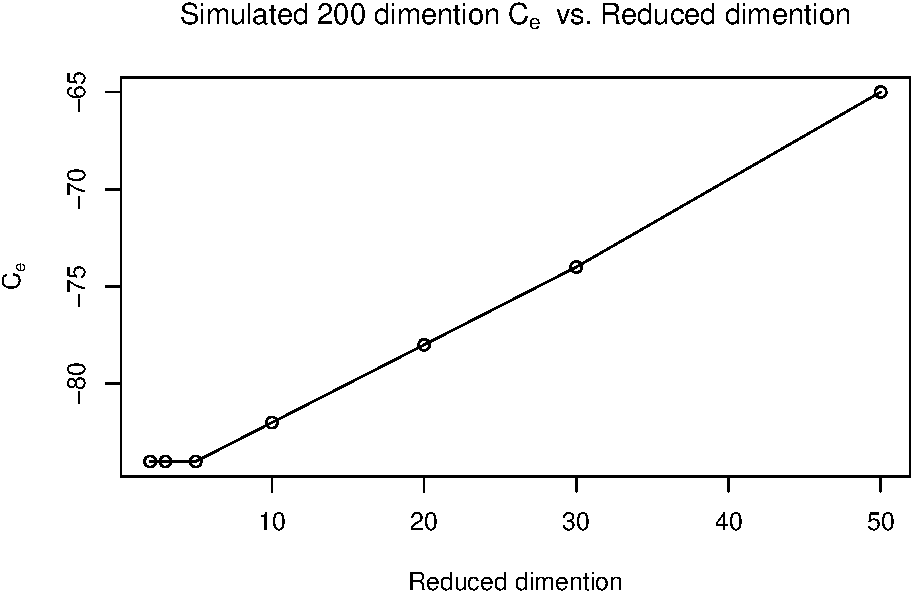
\includegraphics[width=1\linewidth]{Report2_files/figure-latex/unnamed-chunk-3-1} \end{center}

\subsection{Table Sim1000}\label{table-sim1000}

\begin{table}[H]
\centering\rowcolors{2}{gray!6}{white}

\begin{tabular}{rrrr}
\hiderowcolors
\toprule
d & ARI\_p & ARI\_d & C\_e\\
\midrule
\showrowcolors
2 & 0.8233352 & 0.0028831 & -82\\
3 & 0.8233352 & 0.0031754 & -82\\
5 & 0.8233397 & 0.0036920 & -82\\
10 & 0.8233352 & 0.0047544 & -82\\
20 & 0.8233397 & 0.0059592 & -82\\
\addlinespace
30 & 0.8233488 & 0.0076884 & -82\\
50 & 0.8233397 & 0.0103410 & -81\\
\bottomrule
\end{tabular}
\rowcolors{2}{white}{white}
\end{table}

\subsection{Plot Sim1000}\label{plot-sim1000}

\begin{center}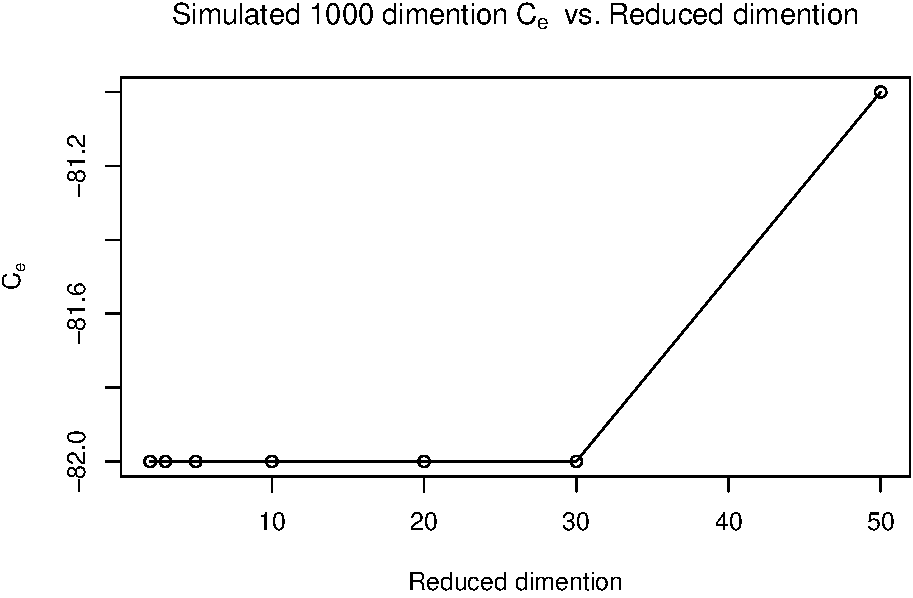
\includegraphics[width=1\linewidth]{Report2_files/figure-latex/unnamed-chunk-5-1} \end{center}

\section{\texorpdfstring{For \(\alpha\) = 1, d(reduced dimention) = 2,3,
5, 10, 20, 30,
50}{For \textbackslash{}alpha = 1, d(reduced dimention) = 2,3, 5, 10, 20, 30, 50}}\label{for-alpha-1-dreduced-dimention-23-5-10-20-30-50}

\subsection{Table Sim200}\label{table-sim200-1}

\begin{table}[H]
\centering\rowcolors{2}{gray!6}{white}

\begin{tabular}{rrrr}
\hiderowcolors
\toprule
d & ARI\_p & ARI\_d & C\_e\\
\midrule
\showrowcolors
2 & 0.8600812 & 0.0127881 & -85\\
3 & 0.8600812 & 0.0125081 & -85\\
5 & 0.8600812 & 0.0135053 & -85\\
10 & 0.8600812 & 0.0135418 & -85\\
20 & 0.8600812 & 0.0134440 & -85\\
\addlinespace
30 & 0.8600812 & 0.0139522 & -85\\
50 & 0.8600812 & 0.0147410 & -85\\
\bottomrule
\end{tabular}
\rowcolors{2}{white}{white}
\end{table}

\subsection{Plot Sim200}\label{plot-sim200-1}

\begin{center}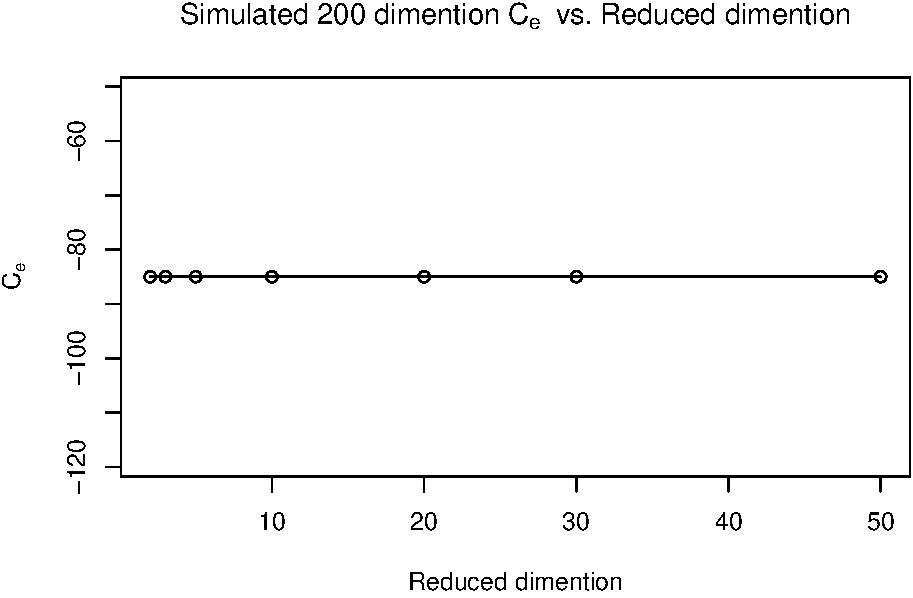
\includegraphics[width=1\linewidth]{Report2_files/figure-latex/unnamed-chunk-8-1} \end{center}

\subsection{Table Sim1000}\label{table-sim1000-1}

\begin{table}[H]
\centering\rowcolors{2}{gray!6}{white}

\begin{tabular}{rrrr}
\hiderowcolors
\toprule
d & ARI\_p & ARI\_d & C\_e\\
\midrule
\showrowcolors
2 & 0.8233352 & 0.0027118 & -82\\
3 & 0.8233352 & 0.0027245 & -82\\
5 & 0.8233352 & 0.0025270 & -82\\
10 & 0.8233397 & 0.0027831 & -82\\
20 & 0.8233352 & 0.0027944 & -82\\
\addlinespace
30 & 0.8233397 & 0.0026015 & -82\\
50 & 0.8233352 & 0.0026218 & -82\\
\bottomrule
\end{tabular}
\rowcolors{2}{white}{white}
\end{table}

\subsection{Plot Sim1000}\label{plot-sim1000-1}

\begin{center}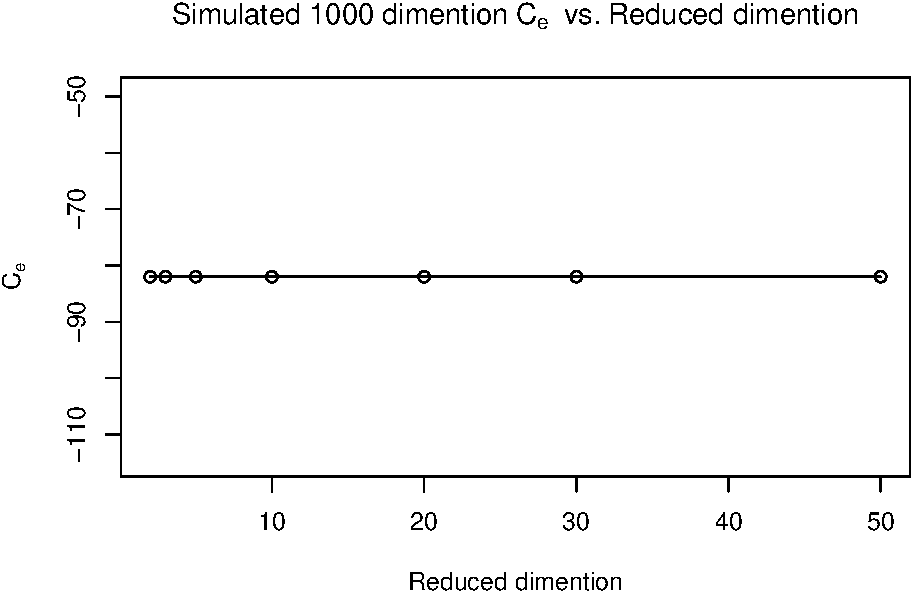
\includegraphics[width=1\linewidth]{Report2_files/figure-latex/unnamed-chunk-10-1} \end{center}

\section{For s = 2, d(reduced dimention) = 2,3, 5, 10, 20, 30,
50}\label{for-s-2-dreduced-dimention-23-5-10-20-30-50}

\subsection{Table Sim200}\label{table-sim200-2}

\begin{table}[H]
\centering\rowcolors{2}{gray!6}{white}

\begin{tabular}{rrrr}
\hiderowcolors
\toprule
d & ARI\_p & ARI\_d & C\_e\\
\midrule
\showrowcolors
2 & 0.8600812 & 0.0175178 & -84\\
3 & 0.8600812 & 0.0198378 & -84\\
5 & 0.8600812 & 0.0262968 & -83\\
10 & 0.8600812 & 0.0407918 & -82\\
20 & 0.8600812 & 0.0816119 & -78\\
\addlinespace
30 & 0.8600812 & 0.1240261 & -74\\
50 & 0.8600812 & 0.2177254 & -64\\
\bottomrule
\end{tabular}
\rowcolors{2}{white}{white}
\end{table}

\subsection{Plot Sim200}\label{plot-sim200-2}

\begin{center}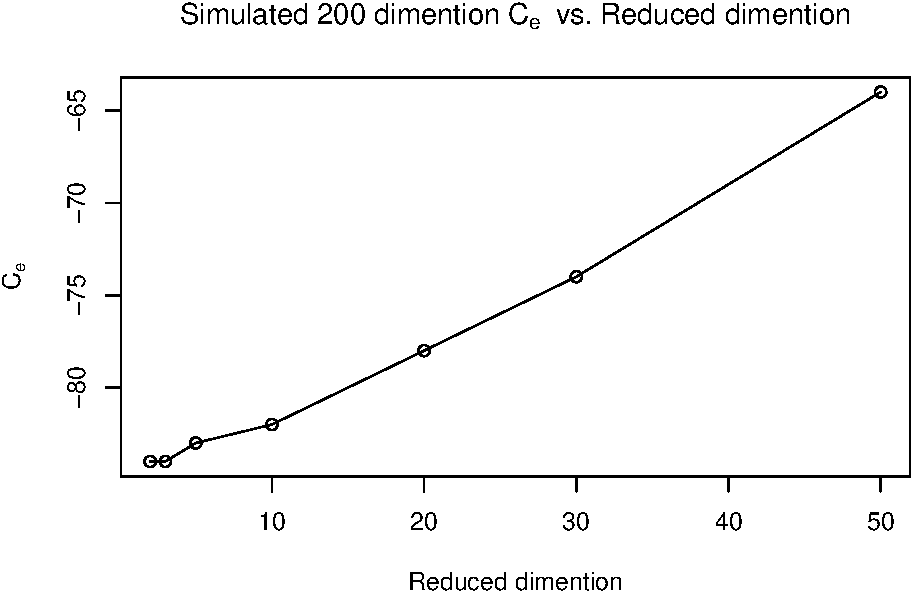
\includegraphics[width=1\linewidth]{Report2_files/figure-latex/unnamed-chunk-13-1} \end{center}

\subsection{Table Sim1000}\label{table-sim1000-2}

\begin{table}[H]
\centering\rowcolors{2}{gray!6}{white}

\begin{tabular}{rrrr}
\hiderowcolors
\toprule
d & ARI\_p & ARI\_d & C\_e\\
\midrule
\showrowcolors
2 & 0.8233352 & 0.0028570 & -82\\
3 & 0.8233352 & 0.0032665 & -82\\
5 & 0.8233352 & 0.0034172 & -82\\
10 & 0.8233443 & 0.0049866 & -82\\
20 & 0.8233352 & 0.0057479 & -82\\
\addlinespace
30 & 0.8233443 & 0.0071553 & -82\\
50 & 0.8233352 & 0.0099807 & -81\\
\bottomrule
\end{tabular}
\rowcolors{2}{white}{white}
\end{table}

\subsection{Plot Sim1000}\label{plot-sim1000-2}

\begin{center}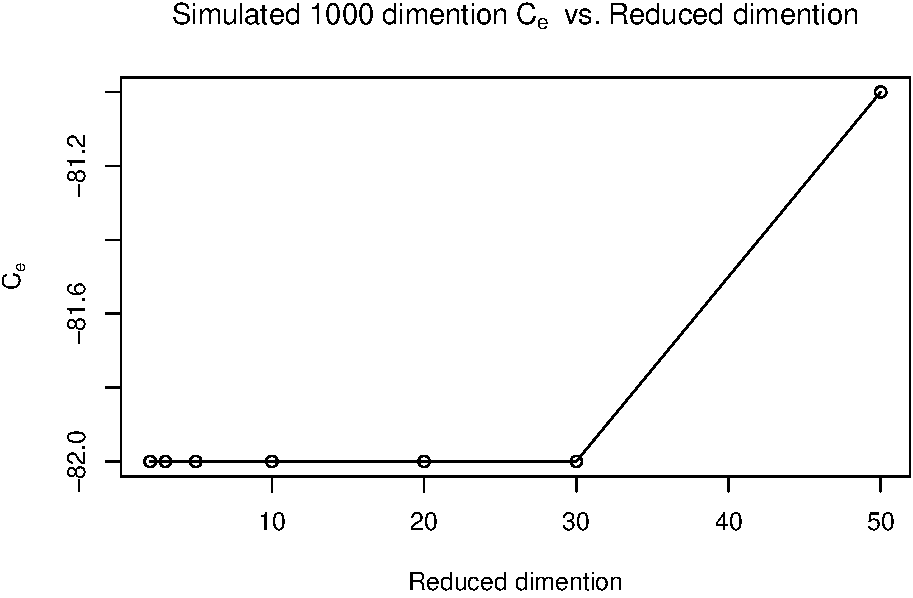
\includegraphics[width=1\linewidth]{Report2_files/figure-latex/unnamed-chunk-15-1} \end{center}


\end{document}
